\lhead{\emph{\leftmark}} 
\chapter{Reverse Engineering of Object Oriented Systems into Umple}
\label{chap:core}

In this chapter we provide an overview of our reverse-engineering technique, called \textit{umplification}. Then, we discuss our motivations for developing the umplification technique and present a comprehensive example. 

\section{Umplification Process}

\textit{Umplification} is a play on words with the concept of 'amplification' and also the notion of converting into Umple. The techniques produces a program with behavior identical to the original one, but written in Umple. The umplification process is incrementally performed until the desired level of abstraction is achieved. 

\subsection{Description}
Umplification, as illustrated in Figure \ref{fig:umplificationLoop}, involves recursively modifying the Umple model/code or the base language code to incorporate additional abstractions, while maintaining the semantics of the program, and also maintaining, to the greatest extent possible, such elements as layout. The end product of umplification is an Umple program/model that can be edited and viewed textually just like the original program, and also diagrammatically, using Umple's tools. 

\begin{figure}[h]
\centering
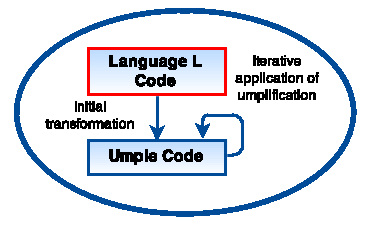
\includegraphics[width=0.50\textwidth]{Figures/UmplificationProcess.pdf}
\caption{The Umplification process generalized}
\label{fig:umplificationLoop}
\end{figure}

% I would get rid of the red double-arrowed arc. It is confusing. Also make the blue double-arrowed arc into a single-arrowed arc
% MG FIXED

\subsection{Properties}

The umplification process has several properties. It is:
\begin{enumerate}
 \item \textbf{incremental}, 
 \item \textbf{transformational},
 \item \textbf{interactive},  
 \item \textbf{extensible}, and
 \item \textbf{implicit-knowledge} conserving. 
\end{enumerate}

The approach is \textbf{incremental} because it can be performed in multiple small steps that produce (quickly) a new version of the system that has a small amount of additional modeling information, such as the presence of one new type of UML/Umple construct. At each step, the system remains compilable. The approach proceeds incrementally performing additional transformations until the desired level of abstraction is achieved.	These incremental transformations allow for user interaction to provide needed information that may be missing or hard to automatically obtain because the input (the source code) does not follow any of the idioms the automatic umplification tool is yet able to recognize. This characteristic of umplification allows developers, if they wish, to repeatedly re-introspect the transformed program and manually validate each change with an understanding of the incremental purpose of the change.

The approach is \textbf{transformational} because it modifies the original source rather than generating something completely new. It first translates the original language (Java, C++ etc.) to an initial Umple version that looks very much like the original, and then translates step-by-step as more and more modeling constructs are added, replacing original code.

The approach is \textbf{interactive} because the user's feedback may be used to enhance the transformations.

The approach is \textbf{extensible} because it uses the set of transformation rules can be readily extended to refine the transformation mechanism. 

Finally the approach is \textbf{implicit-knowledge} conserving because it preserves code comments, and, where possible, the layout of whatever code is not (yet) umplified. The latter includes as the bodies of algorithmic methods – known as \textit{action code} in UML.

Taken together, the above properties allow developers to confidently umplify their systems without worrying about losing their mental model of the source code. Developers gain by having systems with a smaller body of source code that is intrinsically self-documented in UML. 

\subsection{Overview of Transformations cases}

The following gives a summary of the abstract transformations currently implemented. 
\begin{description} 
\item[Transformation 0: Initial transformation] 
Source files written in language L (e.g. Java, C++) code are initially renamed as Umple files, with extension .ump. File, package and data type dependencies are translated into Umple dependencies by using the Umple depend construct. 

\item [Transformation 1: Transformation of generalization/specialization, and namespace declarations]
The notation in the base language code for subclassing is transformed into the Umple 'isA' notation. Umple now recognizes the class hierarchy. Notations for namespaces or packages are transformed into the Umple 'namespace' directives. At this stage, an Umple program, when compiled should generate essentially identical code to the original program.

\item [Transformation 2: Analysis and conversion of many instance variables, along with the methods that use the variables]
This transformation step is further decomposed into sub-steps depending on the abstract use of the variables. The sub-steps are defined as follows.
	\begin{description}

	\item [Transformation 2a: Transformation of variables to UML/Umple attributes]
	If variable \textit{a} is declared in class A and the type of \textit{a} is one of the primitive types in the base language, then \textit{a} is transformed into an Umple attribute. Any accessor (e.g. getA()) and mutator (e.g. setA(…)) methods of variable a are transformed as needed to maintain a functioning system. In particular, any getter and setter methods in the original system must be adapted to conform to or call the Umple-generated equivalents.
	
	\item [Transformation 2b: Transformation of variables in one or more classes to UML/Umple associations]
	If variable \textit{a} is declared in Class A and the type of \textit{a} is a reference type B, then a is transformed into an Umple Association with ends \{a, b\}. At the same time, if a variable b in class B is detected that represents the inverse relationship then the association becomes bidirectional. The accessor and mutator methods of variable \textit{a} (and \textit{b}) are adapted to conform to the Umple-generated methods. Multiplicities and role names are recovered by inspecting both types A and B;

	\item [Transformation 2c: Transformation of variables to UML/Umple state machines]
	If \textit{a} is declared in Class A, has not been classified previously as an attribute or association, has a fixed set of values, and changes in the values are triggered by events, and not by a set method, then a is transformed to a state machine.	
%We will not cover this aspect of umplification further in this thesis, and will leave the focus on attributes and associations.
% If time allows, state machines will be cover since I have some rules for it.
% TL: I suggest covering it lightly, indicating that further investigation is future work
\end{description}
\end{description}

As mentioned before, as part of each transformation step, the accessor, mutator, iterator and event methods are adapted (refactored) to conform to the Umple generated methods. Table \ref{table:transformations} summarizes these additional required refactorings. 

\begin{table}[htbp]
	\caption{Refactorings to methods required for each transformation}
	\label{table:transformations}
    \centering
    \begin{tabularx}{\textwidth}{| X | X |}
        \toprule
        \rowcolor[HTML]{BBDAFF}
       \textbf{ Transformation case  }   & \textbf{Method Transformations}
        \\ \hline
        \textbf{(0)  Classes }        & None      \\ \hline
        \textbf{(1)  Inheritance}     & None       \\ \hline
        \textbf{2a)  Attributes}      & 
        Accessor (getter) and mutator (setter) methods are removed from the original code if they are simple since 		Umple-generated code replaces them. Custom accessors and mutators are refactored so Umple generates code 			that maintains the original
        semantics.         		\\ \hline
        \textbf{(2b) Associations }   & 
 		Accessor and mutator methods are removed or correctly injected into the Umple code.        
		\\ \hline
        \textbf{(2c) State Machines  }  & 
		Methods triggering state change are removed if they are simple (just change state) or modified to call 				Umple-generated event methods.  	
		\\ \hline
    \end{tabularx}
\end{table}

In the following section, we provide a more detailed view of the transformation cases and an example to summarize the main points of the umplification process. To help distinguish between Umple and Java code presented in this thesis, the Umple examples appear in solid borders with blue shading, pure Java examples have solid borders with green shading. 

\subsubsection{More Details of the Initial Transformation}

As mentioned, the first step in umplification (Transformation 0) is to rename the Java/C++ files as .ump files.

After this, various syntactic changes are made (Transformation 1) to adapt the code to Umple's notations for various features that are expressed differently in Java and C++. Umple maintains its own syntax for these features so as to be language-independent.
First the base language notation for inheritance (e.g. `extends' in Java) or interface implementation (e.g. `implements') is changed into the Umple notation 'isA'. This Umple keyword is used uniformly to represent the generalization relation-ship for classes, interfaces and traits. The same notation is used for all three for flexibility – so that, for example, an interface can be converted to a class with no change to its specializations, or a trait can be generated as a superclass in languages such as C++ where multiple inheritance is allowed.

After this, the dependency notation in the native language (e.g. 'import' in Java) is changed to the 'depend' notation in Umple. Finally 'package' declarations are transformed into Umple namespace declarations. 
Transformations made as part of these first refactoring steps, are one-to-one direct and simple mappings between constructs in the base language and Umple. No methods need changing. The final output after execution of the above transformations, is an Umple model/program that can be compiled in the same manner as the original base language code. At this point, any available test cases may be run to ensure that the program's semantics are preserved.

\subsubsection{Details of the Transformations to Create Attributes}

The goal of this step is to transform member variables meeting certain conditions into Umple attributes (Transformation 2a). An Umple attribute, as discussed in Chapter 2, it is more than just a plain private variable: It is designed to be exclusively operated on by mutator methods, accessed by accessor methods and (depending on its properties) automatically initialized in the constructor. These methods, in turn can have semantics such as preconditions and tracing injected into them. 

We start by analyzing all instance variables for their presence in constructor and get/set methods and decide whether the member variable is a good candidate to become an Umple attribute. In addition to the previous conditions, if the candidate attribute has as its type either:

\begin{enumerate}
\item a simple data type
\item a class that only itself contains instance variables meeting conditions in a and b (for attributes with 'many' multiplicity)
\end{enumerate}

Then, the member variable is transformed into an Umple Attribute. If it is not possible to draw a conclusion regarding whether or not the member variable corresponds to an Umple Attribute, the member variable is left to be later transformed into an association or a state machine. If the member variable does not meet any of the criteria required to perform the transformations, the member variable (and its accessors/mutators) is not processed. Further details on this decision making process will be provided in the next chapter of this thesis. 

We culminate this refactoring step by removing or refactoring getters and setters of the previously identified attributes. More specifically, the getters and setters need to be refactored if they are custom. Simple getters/setters are those that only return/update the attribute value.  Custom getters/setters are those that provide behavior apart from getting and setting the variable such as validating constraints, managing a cache or filtering the input.

\subsubsection{Transformations to Create Associations}

As discussed earlier, in the various cases of the refactoring steps, analyses are applied to the input variables to determine whether each variable can be transformed into an Umple association. An association specifies a semantic relationship that occurs between typed instances. A variable represents an association if all of the following conditions apply:

\begin{itemize}
\item Its declared type is a Reference type (generally a class in the current system).
\item The variable field is simple, or the variable field is a container (also known as a collection).
\item The class in which the variable is declared, stores, access and/or manipulates instances of the variable type.

% You had a duplication of the last bullet, which I took out, however is it possible there was originally some different 4th item?
% MG. Three items only, last one was duplicated.

\end{itemize}

The sort of refactoring discussed above for attributes is also performed when associations are found, although the actual code logic is more sophisticated.

A complete analysis on the different transformations cases is presented in Chapter \ref{chap:detections}. From this analysis, a set of transformations rules are derived. The actual implementation of the transformations rules is discussed in Chapter \ref{chap:tool}.

% Here you should add a forward reference to where you will talk about the actual rules and mechanism used to do the transformations. You should also mention state machines I think
% MG Done

\section{Motivations}

Our desire to develop our reverse-engineering approach arose for two main reasons. We address each of these in the following sections.

\subsection{Model-code duality}

Developers often work with large volumes of legacy code. Reverse engineering tools allow them to extract models in a variety of ways \cite{OsmanChaudron}, often with UML as the resulting formalism.

The extracted models can be temporary, just-in-time aids to understanding, to be discarded after being viewed. Such a mode of use can be useful, but is limited in several ways: Developers still need to know where to start exploring the system, and they need to remember how to use the reverse engineering tool every time they perform an exploration task. 

Developers generally therefore would benefit from choosing reverse engineering tools that create a more permanent form of documentation that can be annotated or embedded in larger documents, and serve as the definitive description of the system. 

However by making the latter choice, the developer then needs to maintain two different artifacts, the original code and the output model. The recovered models become obsolete quickly, unless they are continuously updated or are used for 'roundtrip engineering'.  The complexity of this inhibits developers from using reverse engineering tools for permanent documentation.

The umplification technique we present in this thesis overcomes the problems with either mode of reverse engineering described above. It results in a system with a model that can be explored as easily as with just-in-time tools. But there is also no issue with maintaining the model, because model and code become the same thing.

In other words, the key difference compared to existing reverse engineering techniques and the main motivation for this work is that the end-product of umplification is not a separate model, but a single artifact seen as both the model and the code. In the Umple world, modeling is programming and vice versa. More specifically, for a programmer, Umple looks like a programming language and the Umple code can be viewed as a traditional UML diagram. This allows developers to maintain the essential 'familiarity' with their code as they gradually transform it into Umple \cite{Forward2008}. 

\subsection{Improving Program Comprehension}

In addition to solving the problem of having two different software artifacts to maintain,   umplification can be used to simplify a system. The resulting Umple code base tends to be simpler to understand \cite{UmpleMAIN} as the abstraction level of the program has been 'amplified'.

With a system written in Umple, large amounts of boilerplate code are avoided. The benefits of \textit{umplifying} a system not only include recovering a textual model but also eliminating that repetitive code from the programs. For instance, when an association is umplified, all the methods for adding, removing and setting links of the association, are removed (or refactored under certain conditions that will be explained later). This promotes code readability and reduces code volume and code density. Kiczales provides in his work \cite{kiczalesAOP} some evidence that reducing the code volume can help to improve program comprehension.

The Umplification technique improves program comprehension by:
\begin{itemize}
\item Allowing developers to describe and develop a system at a more abstract level and

\item Removing boilerplate code when incorporating a new abstraction

\item Reducing the complexity when an Umple association is incorporated. An Umple association consists of a single line of Umple code. To implement the association in a language like Java, we need to include member variables in both classes, methods to add, delete, query an iterate through links, as well as some code in the constructors.

\item Reducing the complexity when an Umple attribute is incorporated. First, attributes can remain untyped (defaulted to a String implementation) and generate both set/get accessor methods, which further reduces the code volume and code density. Complexity is also significantly reduced since the mechanism to manage a list attribute does not have to be coded. This API includes methods like adding and removing entities, retrieving one or all entities as well as asking how many entities belonging to the instance.
\end{itemize}

\section{School System - Manual Umplification Example}
We illustrate the umplification process with a small example. The original Java is presented through Listings \ref{lst:StudentJava} - \ref{lst:personJava}.

\noindent\begin{minipage}{.45\textwidth}
\begin{lstlisting}[style=java,caption=Student.java,label=lst:StudentJava]{Name}
package university;

public class Student extends Person{ 

 public static final int MAX_PER_GROUP = 10; 
 private int id; 
 private String name;
 public Mentor mentor; 

 public Student(int id,String name){ 
  id = id; name = name; 
 } 
 public String getName(){
  String aName = name;
   if (name == null) { 
    throw new RuntimeException("Error");
   } 
   return aName; 
 }
 public Integer getId() {
  return id;
 }
 public void setId(Integer id) { 
  this.id = id; 
 } 
 public boolean getIsActive() { 
  return isActive;
 }
 public void setIsActive(boolean aIsActive) {
  isActive = aIsActive;} 
 }   
 public Mentor getMentor() { 
  return mentor; 
 }
 public void setMentor(Mentor mentor) { 
  this.mentor = mentor; 
 } 
}
\end{lstlisting}
\end{minipage}\hfill
\begin{minipage}{.45\textwidth}
\begin{lstlisting}[style=java,caption=Mentor.java,label=lst:mentorJava]{Name1}
package university;
import java.util.Set;

public class Mentor extends Person{ 

 Mentor() {}
 public Set<Student> students;
 public Set<Student> getStudents() {
  return students; 
 } 
 public void setStudents (Set<Student>students) { 
  this.students = students;
 } 
 public void addStudent( Student aStudent){
  students.add(aStudent); 
 }
 public void removeStudent(Student aStudent) {
  students.remove(aStudent);
 } 
 public String toString() {
      return(
         (name==null ? " " : name) + " " +
         students.size()+ " students"
      );
 }
}
\end{lstlisting}
\end{minipage}

\begin{lstlisting}[style=java,caption=Person.java,label=lst:personJava]
package university;
public class Person {
 public String getName() {return this.name;}
 public void setName(String name){
  this.name= name;
 }
}
\end{lstlisting}


\subsection{School system: Initial Transformation}

We create the .ump files, one Umple file per input class. Three Umple files, in Listings \ref{lst:mentorUmple}, \ref{lst:studentUmple0},\ref{lst:personUmple0} ,are created as result of this initial transformation. 

% Make a reference to the relevant listings for the three files
% MG Fixed

As discussed earlier, the dependency, package and generalization notation is changed to their respective Umple notation. For instance, the Java code of class Mentor shown in Listing \ref{lst:mentorJava} would result in  Umple implementation shown in Listing  \ref{lst:mentorUmple} (in file Mentor.ump). The following give details of the initial transformation:

\begin{itemize}
\item Package declaration in \ref{lst:mentorJava} becomes an Umple namespace declaration in Listing \ref{lst:mentorUmple}.
\item Import declaration in \ref{lst:mentorJava} becomes an Umple depend declaration in Listing \ref{lst:mentorUmple}.
\item Generalization notation in \ref{lst:mentorJava} is transformed to the 'isA' notation (Line 5) in Listing \ref{lst:mentorUmple}.
\item Code in Lines 6-26 in Listing \ref{lst:mentorJava} is not touched by the initial trasnformation; The same exact code is found in the Umple file in Listing \ref{lst:mentorUmple} (Lines 7-27).
\end{itemize}

\begin{lstlisting}[style=UmpleIn,caption=Mentor.ump,label=lst:mentorUmple]
namespace university;
class Mentor { 

 depend java.util.Set;
 isA Person;
 
 Mentor() {}
 public Set<Student> students;
 public Set<Student> getStudents() {
  return students; 
 } 
 public void setStudents (Set<Student>students) { 
  this.students = students;
 } 
 public void addStudent( Student aStudent){
  students.add(aStudent); 
 }
 public void removeStudent(Student aStudent) {
  students.remove(aStudent);} 
 } 
 public String toString() {
      return(
         (name==null ? " " : name) + " " +
         students.size()+ " students"
      );
 }
}
\end{lstlisting}

The umple code for classes Student and Person after completion of the first refactoring step is presented in Listings \ref{lst:studentUmple0} and \ref{lst:personUmple0}. 

\begin{lstlisting}[style=UmpleIn,caption=Student.ump,label=lst:studentUmple0]
namespace university;
class Student {
 isA Person;
 public static final int MAX_PER_GROUP = 10; 
 private int id; 
 private String name;
 public Mentor mentor; 

 public Student(int id,String name){ 
  id = id; name = name; 
 } 
 public String getName(){
  String aName = name;
   if (name == null) { 
    throw new RuntimeException("Error");
   } 
   return aName; 
 }
 public Integer getId() {
  return id;
 }
 public void setId(Integer id) { 
  this.id = id; 
 } 
 public boolean getIsActive() { 
  return isActive;
 }
 public void setIsActive(boolean aIsActive) {
  isActive = aIsActive;} 
 }   
 public Mentor getMentor() { 
  return mentor; 
 }
 public void setMentor(Mentor mentor) { 
  this.mentor = mentor; 
 } 
}
\end{lstlisting}

\begin{lstlisting}[style=UmpleIn,caption=Person.ump,label=lst:personUmple0]
namespace university;
class Person { 
 public String getName() {return this.name;}
 public void setName(String name){
  this.name= name;
 }
}
\end{lstlisting}

The visual representation of the Umple model at the end of this transformation step is shown in Figure \ref{fig:Example1a1}. At this point, we have gained knowledge about the hierarchical structure of the system. Attributes and associations are not shown in the diagram since they have not been yet reverse-engineered.

\begin{figure}[h]
\centering
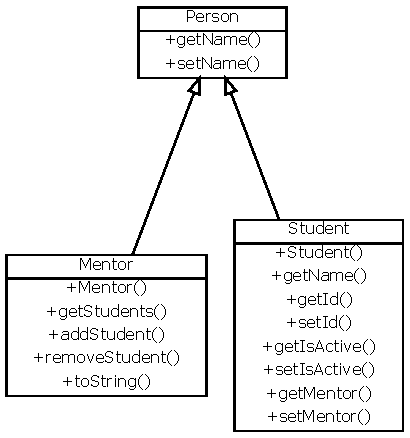
\includegraphics{Figures/Example1a1.pdf} 
\caption{UML Class Diagram of the Mentor-Student example - Level 1}
\label{fig:Example1a1}
\end{figure}

\subsection{School system: Transformations to Create Attributes}

Assuming that we have successfully performed the initial transformation on all the input files, at this point the input for the second transformation step are three Umple files.
We first analyze the variables (they are still variables even if they are inside an Umple class) to determine certain characteristics such as the following:

\begin{enumerate}
\item Is the field present in the parameters of the constructor?
\item Does the field possess a getter?
\item Does the field possess a setter?
\item Is the field's type, a primitive type?
\end{enumerate}

For instance, if we analyze the member variables in class Student, we obtain the results in Table \ref{table:analysisStudent}.

\begin{table}[ht]
\caption{Analysis of Member variables of class Student}
\label{table:analysisStudent}
\centering
\begin{tabular}{l|cccc}
\toprule
\rowcolor[HTML]{BBDAFF}
\textbf{Member Variable} & \textbf{1}  & \textbf{2}   & \textbf{3}   & \textbf{4}    \\ \hline
id & Yes &  Yes &  Yes &  Yes \\ 
isActive &  No &  Yes &  Yes &  Yes \\ 
name &  Yes &  Yes &  No &  Yes \\ 
MAX\_PER\_GROUP &  No &  No &  No &  Yes \\ 
\hline
\end{tabular}
\end{table}

% The above table does not exist.
% MG. Table Added 

The results of this analysis allow us to generate Umple code with the required types and stereotypes. For example the stereotype 'lazy' is added to 'isActive' because it should not appear in the constructor, and the stereotype `immutable' is added to \textit{name} since there is no setter. The transformed Umple code after completion of this refactoring step (transformation 2a) is shown in Listing \ref{lst:studentUmple}. Note that this continues to generate a program that is semantically identical to the pre-transformation version.

\begin{lstlisting}[style=UmpleOut,caption=Student.ump,label=lst:studentUmple]
namespace university;

class Student { 
 Integer id; 
 lazy Boolean isActive; 
 immutable name; 
 const Integer MAX_PER_GROUP = 10; 
 after getName {
  if (name == null) { 
   throw new RuntimeException("Error");
  }
 }
  public Mentor mentor; 
  public Mentor getMentor() { 
   return mentor; 
  }
  public void setMentor(Mentor mentor) { 
   this.mentor = mentor; 
  } 
}
\end{lstlisting}

% I am confused by the colours. The colour of this background is light blue. The colour of the previous listing is dark blue-grey, but they are both Umple.
% MG. Fixed for now, with two colors only: one for umple, one for java.
% MG. Will be enhanced later, with titles in the boxes as in Ahmed's thesis.

The following gives details of Listing \ref{lst:studentUmple}:
\begin{itemize}
\item Line 4: Field id becomes an Umple attribute. Getter getId() and setter setId() are removed.

% line numbers are off by 2 in these items
% MG Fixed.
\item Line 5: Field isActive becomes an Umple attribute of Boolean type.  As the field is not required in the constructor we marked as 'lazy' so the Umple compiler does not generate a constructor argument for this attribute. 

\item Line 6: Field name becomes an Umple attribute and is marked as 'immutable'. Immutable attributes must be specified in the constructor, and no setter is provided. In this particular example, the input java code (Listing \ref{lst:StudentJava}) does not contain code that sets this variable anywhere, therefore it is transformed into an immutable umple attribute. 

% explain why we would know this should be immutable - you find no code that sets it anywhere.
% MG. Explanation addded in paragraph above.
\item Line 7: Field MAX\_PER\_GROUP becomes a constant (special type of Umple attribute). We have drawn this conclusion because of the field modifiers (e.g. static final) and because of the ALL\_CAPS convention. 

\item Line 8-12: As the getter for field name was custom in Listing \ref{lst:StudentJava}, we have adapted it so it conforms to the one that can be generated by the Umple compiler. A code injection, code that is injected before and/or after statements, have been used for this purpose.

\item Code in Lines 32-37 in Listing \ref{lst:StudentJava} is not touched by this transformation; The same exact code is found in the Umple file in Listing \ref{lst:studentUmple} (Lines 13-19).
% reference to lst:studentJava not resolved above.
% MG Fixed.

\end{itemize}

In the same manner, we umplify the attributes of classes Mentor and Person.
The Umple code for class Mentor remains identical as in Listing \ref{lst:mentorUmple}, since we could not find any member variables in this class meeting the conditions to become an Umple attribute. On the other hand, the member variable 'name' in class Mentor has been transformed into an attribute of String type. The resulting Umple code for class Person, after this transformation is shown below in Listing \ref{lst:personUmple}.

\begin{lstlisting}[style=UmpleOut,caption=Person.ump,label=lst:personUmple]
namespace university;
class Person {
 String name;
}
\end{lstlisting}

The visual representation of the Umple model at the end of this transformation step is shown in Figure \ref{fig:Example1a2}. At this point, we have gained knowledge about the hierarchical structure of the system and the attributes of each class. Associations are not shown in the diagram since they have not been yet reverse-engineered.

\begin{figure}[h]
\centering
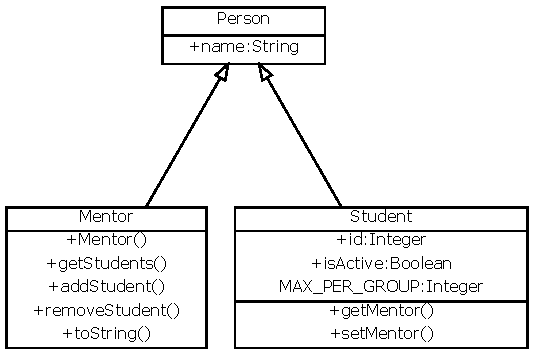
\includegraphics{Figures/Example1a2.pdf} 
\caption{UML Class Diagram of the Mentor-Student example - Level 2}
\label{fig:Example1a2}
\end{figure}

\subsection{School system: Transformations to Create Associations}

Assume again that the source code has already passed through the two first refactoring steps and the input at this point is the Umple code found in Listings \ref{lst:personUmple}, \ref{lst:mentorUmple} and \ref{lst:studentUmple}.

The resulting Umple code for class Mentor after completion of this refactoring step (transformation 2b) is shown below in Listing \ref{lst:mentorUmple2}. Line 2 contains the association derived from the Java code that can be read as: a mentor can have many students associated but a student can only be associated to at most one mentor. 

\begin{lstlisting}[style=UmpleOut,caption=Mentor.ump,label=lst:mentorUmple2]
namespace university;
class Mentor {
 0..1 -- 0..* Student; 
 
 public String toString() {
  return(
  (name==null ? " " : name) + " " +
   students.size()+ " students");
 }
}
\end{lstlisting}

\begin{lstlisting}[style=UmpleOut,caption=Student.ump,label=lst:studentUmple2]
namespace university;
class Student {
 Integer id; 
 lazy Boolean isActive; 
 immutable name; 
 const Integer MAX_PER_GROUP = 10; 
 
 after getName {
  if (name == null) { 
   throw new RuntimeException("Error");
  }
 }
}
\end{lstlisting}

The following particularities have been taken into consideration during the extraction of the association:

In class \textit{Mentor}:
\begin{enumerate}
\item The students variable in class Mentor is of a reference type and possesses a getter and a setter.
\item We inferred the multiplicity of the association end "0..*" by a) inspecting the cardinality of the member, and b) by analyzing the getter/setter of the member variable.
\item We inferred the navigability of the association "--" by inspecting the two classes involved. In this case, each class can access the linked objects of the other class.  The notation "-$>$" would otherwise have been used to represent a unidirectional association. 

% The -> above was rendering wrongly; note how I fixed it. You might need to deal with this elsewhere.
% MG. OK thanks

\item The association end is optional-many because the member is not present as a parameter in the constructor (not required upon construction) of an instance of the class Mentor and because the member represents a collection of elements. 
\end{enumerate}

In class \textit{Student}:
\begin{enumerate}

\item The mentor in class Student is of a Reference type and it possesses a getter and a setter.
\item We inferred the multiplicity of the association end "0..1" by inspecting the constructor of the class Student. It is optional-one because it is not required upon construction of class Student. 
\item Methods \textit{setMentor()} and \textit{getMentor()} are no longer needed in class Student and therefore removed.
\end{enumerate}

Consider again the previous example.  If we inject now the constructor of Listing \ref{lst:studentConstructor} into the Student class, the multiplicity for the association end would become "1" instead of "0..1". 

\begin{lstlisting}[style=java,caption=A new constructor added to Student class,label=lst:studentConstructor]
public Student(Mentor aMentor){
  mentor = aMentor;
}
\end{lstlisting}

Note that in the examples, the Java input made use of generics (templates using '$<>$' syntax) for the specification of a collection of elements. For those cases in which the type of the member variable cannot be directly inferred (in older Java code), we analyze the add/remove methods to determine the type of the element that is added to the collection. We will explore all possible detection mechanisms for associations in Chapter \ref{chap:detections}. Ultimately, each refactoring step should involve testing (running the test suites) to check that the program's semantics are preserved. 

The visual representation of the Umple model at the end of this transformation step is shown in Figure \ref{fig:Example1a3}. As a result,we have gained knowledge about the hierarchical structure of the system, attributes and associations of each class. 

\begin{figure}[h]
\centering
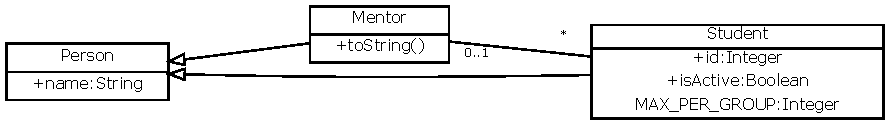
\includegraphics{Figures/Example1a3.pdf} 
\caption{UML Class Diagram of the Mentor-Student example - Level 3}
\label{fig:Example1a3}
\end{figure}

Finally, for this small system, the Umple code extracted (33 LOC) contains substantially fewer lines of code the original system written in Java (77 LOC). Despite being a simple metric, the number of lines of code is a fair indicator of complexity \cite{LOCMetric}. 

\section{ATM system - Manual Umplification Example}

We will now illustrate the transformations steps through an example. This will show how umplification is performed manually. In Chapter 5 we will show how to perform automated umplification.

In this section, we will umplify a moderately-sized Java system  comprised of:

\begin{itemize}
 \item 24 files, 2470 Lines of Code.
 \item Two top packages \textit{atm} and \textit{banking}.
	\begin{itemize}
	 \item atm: ATM, Session
	 \item atm.physical: CardReader, CashDispenser, CustomerConsole, EnvelopeAcceptor, Log, NetworkToBank, OperatorPanel, ReceiptPrinter
	 \item atm.transaction: Transaction, Withdrawal, Deposit, Transfer, Inquiry
	 \item banking: AccountInformation, Balances, Card, Message, Money, Receipt , Status.
	\end{itemize}
 \item Two 'top-level' classes: ATMMain and ATMApplet allowing the system to be run as an application or as an applet.
\end{itemize}

The original Java source code has been taken from \cite{atmsystem}. Although this can be considered as a small application, by going through the source code of the ATM program it is not easy to understand how the classes are organized, how they interact with each other and how the responsibilities are distributed among the classes. A programmer aiming to use, document or extend this ATM application may want to know the impact of a change by looking at the dependencies, generalizations and associations connecting the entities or to obtain a high level view of the system for program understanding. The reader can take any versions of the code, at each step of umplification (obtained from \cite{UmplificationBasicExampleURL}), and paste it into UmpleOnline \cite{UmpleOnline} or our Eclipse-based Umple environment. 

In the following sub-sections, we present the transformation details for the classes in package 'atm.banking' and the main program class for the system 'ATMMain.java'. Note that the comments have been ignored and code in some methods have been omitted to save space.  Listings \ref{lst:CardJava} - \ref{lst:ATMMainJava} present each of the classes in this package, the input code. The Umple code resulting from each step will be shown as well as the UML class diagram (visual representation of the model). 

\noindent\begin{minipage}{.45\textwidth}
\begin{lstlisting}[style=java,caption=Card.java,label=lst:CardJava]{Name}
package banking;

public class Card
{
 private int number;
    
 public Card(int number)
 {
  this.number = number;
 }
    
 public int getNumber()
 {
  return number;
 }   
}
\end{lstlisting}
\end{minipage}\hfill
\begin{minipage}{.45\textwidth}
\begin{lstlisting}[style=java,caption=AccountInfo.java,label=lst:AccountInformation]{Name1}
public class AccountInformation
{
 public static final String [] ACCOUNT_NAMES =
    { "Checking", "Savings", "Money Market" };
         
 public static final String [] ACCOUNT_ABBREVIATIONS =
    { "CHKG", "SVGS", "MMKT" };
}    
\end{lstlisting}
\end{minipage}


\noindent\begin{minipage}{.45\textwidth}
\begin{lstlisting}[style=java,caption=Status.java,label=lst:Status]{Name}
package banking;

public abstract class Status
{
 public String toString()
 {
  if (isSuccess())
   return "SUCCESS";
  else if (isInvalidPIN())
   return "INVALID PIN";
  else
   return "FAILURE " + getMessage();
 }
    
 public abstract boolean isSuccess();
 public abstract boolean isInvalidPIN();
 public abstract String getMessage();
}
\end{lstlisting}
\end{minipage}\hfill
\begin{minipage}{.45\textwidth}
\begin{lstlisting}[style=java,caption=Receipt.java,label=lst:Receipt]{Name1}
package banking;

import atm.ATM;
import atm.transaction.Transaction;
import java.util.Date;
import java.util.Enumeration;

public abstract class Receipt
{

 private String [] headingPortion;
 protected String [] detailsPortion;
 private String [] balancesPortion;  
    
 protected Receipt(ATM atm, Card card, Transaction transaction, Balances   balances)
 {        
  // Code omitted
 }
     
 public Enumeration getLines()
 {
  // Code omitted
 }
}
\end{lstlisting}
\end{minipage}

\noindent\begin{minipage}{.45\textwidth}
\begin{lstlisting}[style=java,caption=Balances.java,label=lst:Balances]{Name}
package banking;

public class Balances
{
 private Money total;
 private Money available;
    
 public Balances(){}
    
 public void setBalances(Money total, Money available)
 {
   this.total = total;
   this.available = available;
 }
    
 public Money getTotal()
 {
  return total;
 }
    
 public Money getAvailable()
 {
  return available;
  }
}
\end{lstlisting}
\end{minipage}\hfill
\begin{minipage}{.45\textwidth}
\begin{lstlisting}[style=java,caption=Money.java,label=lst:Money]{Name1}
package banking;

public class Money
{ 
 private long cents; 
   
 public Money(int dollars)
 {
  this(dollars, 0);
 }
   
 public Money(int dollars, int cents)
 {
  this.cents = 100L * dollars + cents;
 }
    
 public Money(Money toCopy)
 {
  this.cents = toCopy.cents;
 }
    
 public String toString()
 {
  return "$" + cents/100 + 
  (cents %100 >= 10  ? "." + cents % 100 : ".0" + cents % 100);
 }
    
 public void add(Money amountToAdd)
 {
  this.cents += amountToAdd.cents;
 }

 public void subtract(Money amountToSubtract)
 {
  this.cents -= amountToSubtract.cents;
 }

 public boolean lessEqual(Money compareTo)
 {
  return this.cents <= compareTo.cents;
 }
}
\end{lstlisting}
\end{minipage}

\subsection{ATM system: Initial Transformation}
We create the .ump files, one Umple file per input class. 24 Umple files in total (7 for the package 'atm.banking') are created as result of this initial transformation.

The dependency, package and generalization notation is changed to their respective Umple notation.

For instance, the Java code (in file ATMMain.java) shown in Listing  \ref{lst:ATMMainJava} would result in  Umple implementation shown in Listing  \ref{lst:ATMMainUmple} (in file ATMMain.ump). Only the code transformed has been shown in Listings \ref{lst:ATMMainJava} -- \ref{lst:ATMMainJava}. 'The rest of the code' corresponds to the code that has not been touched during the transformation. 

\noindent\begin{minipage}{.45\textwidth}
\begin{lstlisting}[style=java,caption=ATMMain.java,label=lst:ATMMainJava]{Name}
import java.awt.*;
import java.awt.event.*;
import atm.ATM;
import simulation.Simulation;

// Main program  
public class ATMMain
{
   // The rest of the code
}
\end{lstlisting}
\end{minipage}\hfill
\begin{minipage}{.45\textwidth}
\begin{lstlisting}[style=UmpleIn,caption=ATMMain.ump,label=lst:ATMMainUmple]{Name1}
// Main program  
class ATMMain
{
  depend simulation.Simulation;
  depend atm.ATM;
  depend java.awt.event.*;
  depend java.awt.*;
  // The rest of the code
}
\end{lstlisting}
\end{minipage}

At the end of this transformation step, the visual representation of the umplified model is shown in Figure \ref{fig:atmBanking1}.

\subsection{ATM system: Transformations to Create Attributes}

\subsection{ATM system: Transformations to Create Associations}

\section{Summary}

Umplification is a process for converting a base language program into an Umple program, involving a set of transformation steps. Umplification responds to two needs: The first concerns models that become obsolete very quickly. The second is the desire to simplify existing systems.

In this chapter we have discussed the different transformations steps of the Umplification process. In the next Chapter, we will present the mapping rules derived from each of the transformations steps. These transformation rules will be necessary to automate our reverse engineering process. Implementation of the mapping rules are then presented in Chapter \ref{chap:tool}.
